\documentclass[11pt]{article}

% ====================================================
% PACKAGES
% ====================================================
\usepackage[margin=1in, headheight=13.6pt]{geometry}
\usepackage[T1]{fontenc}
\usepackage{lmodern}
\usepackage{microtype}
\usepackage{setspace}
\usepackage{tcolorbox}
\usepackage{amsmath, amssymb, mathtools}
\usepackage{siunitx}
\usepackage{bm}

\usepackage{graphicx}
\usepackage{float}
\usepackage{subcaption}

\usepackage{enumitem}
\usepackage{booktabs}
\usepackage{longtable}
\usepackage{array}
\usepackage{multirow}

\usepackage{xcolor}
\usepackage{hyperref}

\usepackage{fancyhdr}
\usepackage{lastpage}

\usepackage{indentfirst}
\usepackage[justification=centering]{caption}
\usepackage{pdfpages}
\usepackage{listings}

\lstdefinestyle{pystyle}{
    language=Python,
    basicstyle=\ttfamily\small,
    keywordstyle=\color{blue!60!black}\bfseries,
    commentstyle=\color{green!40!black}\itshape,
    stringstyle=\color{orange!70!black},
    numbers=left,
    numberstyle=\tiny\color{gray},
    numbersep=6pt,
    breaklines=true,
    breakatwhitespace=false,
    showstringspaces=false,
    frame=single,
    rulecolor=\color{gray!50},
    tabsize=4
}
\lstset{style=pystyle}

\pagestyle{fancy}
\fancyhf{}
\lhead{\Assignment\ |\ \course}
\rhead{\Name\ |\ \today}
\cfoot{Page \thepage\ of~\pageref{LastPage}}

\hypersetup{
    colorlinks,
    linkcolor={red!50!black},
    citecolor={blue!50!black},
    urlcolor={blue!80!black}
}

\newcommand{\Name}{Arael Anaya}
\newcommand{\Assignment}{Homework 5}
\newcommand{\course}{Robot Mechanics}

% Boxed final-answer environment
\newtcolorbox{result}{
    colback=blue!3!white,
    colframe=blue!40!black,
    boxrule=0.6pt,
    arc=2pt,
    left=6pt, right=6pt, top=4pt, bottom=4pt
}

% Boxed problem-statement environment
\newtcolorbox{statement}{
    colback=gray!5!white,
    colframe=gray!50!black,
    boxrule=0.4pt,
    arc=2pt,
    left=6pt, right=6pt, top=4pt, bottom=4pt
}

% Visible placeholder for work not yet added
\newcommand{\workplaceholder}{%
    \par\vspace{4pt}\noindent\textcolor{gray!60}{\itshape [Work not yet added: paste solution here]}\par\vspace{4pt}%
}

% Boxed correction-note environment (flags a fix made to the original hand calc)
\newtcolorbox{fixnote}{
    colback=orange!5!white,
    colframe=orange!55!black,
    boxrule=0.5pt,
    arc=2pt,
    left=6pt, right=6pt, top=4pt, bottom=4pt,
    fontupper=\small
}

% Notation macros (matching course conventions)
\newcommand{\T}{\bm{T}}
\newcommand{\R}{\bm{R}}
\newcommand{\dvec}{\bm{d}}
\newcommand{\framen}[1]{\{#1\}}
\newcommand{\khat}{\widehat{\bm{k}}}
\newcommand{\wvec}{\bm{\omega}}
\newcommand{\xivec}{\bm{\xi}}
\newcommand{\vvec}{\bm{v}}
\newcommand{\Omvec}{\bm{\Omega}}
\newcommand{\Rotx}{\operatorname{Rot}_x}
\newcommand{\Roty}{\operatorname{Rot}_y}
\newcommand{\Rotz}{\operatorname{Rot}_z}
\newcommand{\atantwo}{\operatorname{atan2}}
\newcommand{\skewx}[1]{\left[#1\right]_{\times}}

\begin{document}


% ====================================================
% PROBLEM 1
% ====================================================
\section*{Problem 1}

\begin{statement}
The ABB arm has the following DH table.
\begin{center}
\begin{tabular}{c | c | c | c | c}
\hline
 Link & $a$ & $d$ & $\alpha$ & $\theta$\\  \hline
 $1$ & $0$   & $d_1$ & $\pi/2$  & $\star$ \\
 $2$ & $a_2$ & $0$   & $0$      & $\star$ \\
 $3$ & $a_3$ & $0$   & $-\pi/2$ & $\star$ \\
 $4$ & $0$   & $d_4$ & $\pi/2$  & $\star$ \\
 $5$ & $0$   & $0$   & $-\pi/2$ & $\star$ \\
 $6$ & $0$   & $d_6$ & $0$      & $\star$ \\ \hline
\end{tabular}
\end{center}
\begin{enumerate}[label=(\alph*), leftmargin=1.6em, itemsep=2pt]
    \item Draw the zero-angle configuration.
    \item Solve the inverse kinematics (show all your work).
    \item How many possible solutions exist?
    \item Write a MATLAB code to demonstrate the efficacy of your script over 100 random test cases.
\end{enumerate}
\end{statement}

\subsection*{Part (a)}
Evaluating the DH table with all $\theta_i = 0$ (see \hyperref[app:code:problem1fig]{\texttt{Problem1Figure.m}, Appendix A}):
\begin{center}
    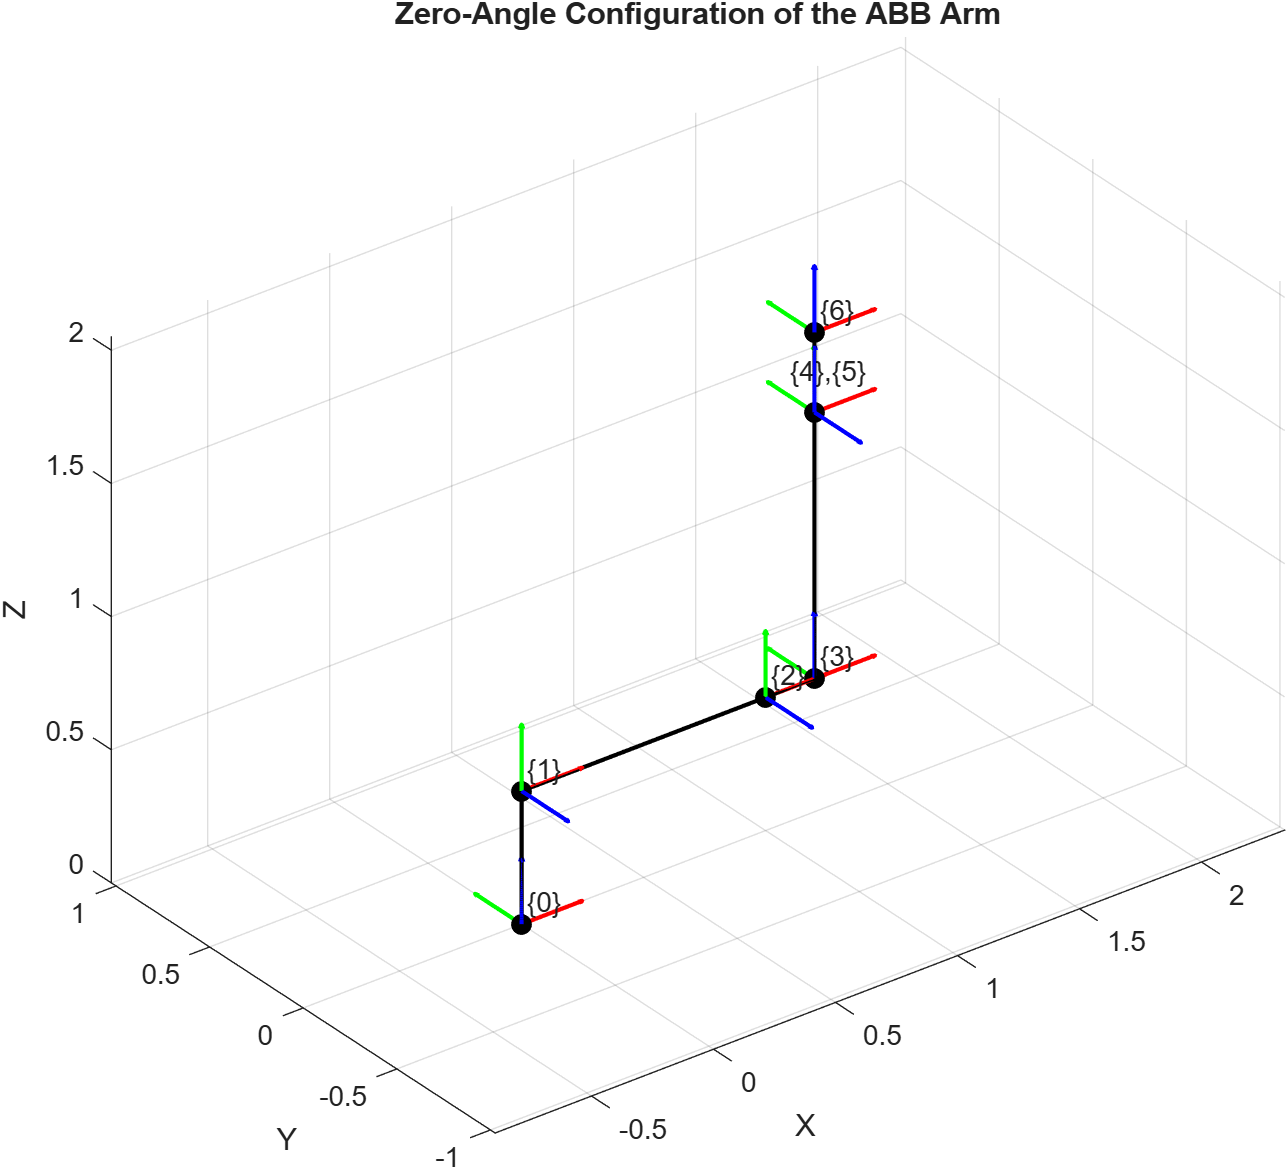
\includegraphics[width=.7\columnwidth]{Figures/Problem1Figure.png}
    \captionof{figure}{Zero-angle configuration of the ABB arm. Axes: $x$ red, $y$ green, $z$ blue. Dimensions are illustrative and differ from Part (d) ($d_1=0.5$, $a_2=1$, $a_3=0.2$, $d_4=1$, $d_6=0.3$). Frames $4$ and $5$ share an origin, so they carry one combined label.}
\end{center}

\subsection*{Part (b)}
The last three axes intersect at the wrist center (origin of frames $\framen{4}$ and $\framen{5}$), so the position and orientation problems decouple.
Let $\bm{P}_{06}=[P_{6x},\,P_{6y},\,P_{6z}]^{\mathsf T}$ and let $\R=\prescript{0}{}{\R}_6$ be the desired orientation. The wrist center is
\begin{equation}
\bm{P}_{05} = \begin{bmatrix}P_{5x}\\P_{5y}\\P_{5z}\end{bmatrix} = \bm{P}_{06} - d_6\,\R(:,3).
\end{equation}

\paragraph{Joint 1.} The projection of $\bm{P}_{05}$ onto the $x_0$--$y_0$ plane lies at angle $\theta_1$ from $x_0$, so
\begin{equation}
\theta_1 = \atantwo\!\left(P_{5y},\,P_{5x}\right) \quad\text{or}\quad \theta_1+\pi.
\end{equation}

\paragraph{Joints 2 and 3.} With $\theta_1$ known, the arm reduces to a planar two-link problem in the plane of $\bm{P}_{05}$. Define
\begin{align}
r &= \sqrt{P_{5x}^2+P_{5y}^2}, \\
D &= \sqrt{P_{5x}^2+P_{5y}^2+(P_{5z}-d_1)^2}, \\
L &= \sqrt{a_3^2+d_4^2},
\end{align}
where $D$ is the distance from $O_1$ to the wrist center and $L$ is the distance from $O_2$ to the wrist center. The pose is reachable only if $|a_2-L|\le D\le a_2+L$. Let $\psi$ be the elevation angle of $D$ above the horizontal and $\beta\in[0,\pi]$ the interior angle at $O_1$ between $a_2$ and $D$. For $\theta_1$ the horizontal reach is $r$; for $\theta_1+\pi$ the arm points the other way, so $r$ is replaced by $-r$:
\begin{equation}
\psi = \atantwo\!\left(P_{5z}-d_1,\; \pm r\right) \quad (+r \text{ for } \theta_1,\; -r \text{ for } \theta_1+\pi), \qquad \theta_2 = \psi \pm \beta .
\end{equation}
Law of cosines on the triangle with sides $a_2$, $D$, $L$:
\begin{align}
L^2 &= a_2^2 + D^2 - 2a_2 D\cos\beta, \\
\cos\beta &= \frac{a_2^2+D^2-L^2}{2a_2D}, \qquad
\sin\beta = +\sqrt{1-\cos^2\beta}, \\
\beta &= \atantwo\!\left(\sqrt{1-\left(\tfrac{a_2^2+D^2-L^2}{2a_2D}\right)^{2}},\; \tfrac{a_2^2+D^2-L^2}{2a_2D}\right).
\end{align}
The only sign choice is the $\pm$ in $\theta_2=\psi\pm\beta$:
\begin{equation}
\theta_2 = \atantwo\!\left(P_{5z}-d_1,\; \pm r\right) \pm \atantwo\!\left(\sqrt{1-\left(\tfrac{a_2^2+D^2-L^2}{2a_2D}\right)^{2}},\; \tfrac{a_2^2+D^2-L^2}{2a_2D}\right).
\end{equation}

For $\theta_3$, let $\delta$ be the fixed angle at $O_2$ between $a_3$ (the segment $O_2\to O_3$) and $L$ (the segment $O_2\to$ wrist center), and $\gamma$ the interior angle at $O_2$ between $a_2$ and $L$:
\begin{equation}
\delta = \atantwo\!\left(d_4,\,a_3\right).
\end{equation}
Law of cosines on the same triangle, now for the angle opposite $D$:
\begin{align}
D^2 &= a_2^2 + L^2 - 2a_2L\cos\gamma, \\
\cos\gamma &= \frac{a_2^2+L^2-D^2}{2a_2L}, \qquad
\sin\gamma = +\sqrt{1-\cos^2\gamma}, \\
\gamma &= \atantwo\!\left(\sqrt{1-\cos^2\gamma},\;\cos\gamma\right).
\end{align}
The elbow sign of $\theta_3$ is tied to the sign of $\beta$ in $\theta_2$:
\begin{equation}
\theta_3 = \mp(\pi-\gamma) - \delta ,
\end{equation}
with the upper sign paired with $\theta_2=\psi+\beta$ (elbow up) and the lower sign with $\theta_2=\psi-\beta$ (elbow down). Explicitly,
\begin{equation}
\theta_3 = \mp\left[\pi - \atantwo\!\left(\sqrt{1-\left(\tfrac{a_2^2+L^2-D^2}{2a_2L}\right)^{2}},\; \tfrac{a_2^2+L^2-D^2}{2a_2L}\right)\right] - \atantwo\!\left(d_4,\,a_3\right).
\end{equation}

\paragraph{Joints 4, 5, and 6.} From the DH table, $\prescript{0}{}{\R}_3$ depends only on $\theta_1,\theta_2,\theta_3$:
\begin{equation}
\prescript{0}{}{\R}_3 = \Rotz(\theta_1)\,\Rotx(\tfrac{\pi}{2})\,\Rotz(\theta_2+\theta_3)\,\Rotx(-\tfrac{\pi}{2}) = \Rotz(\theta_1)\,\Roty\!\big(-(\theta_2+\theta_3)\big).
\end{equation}
Then
\begin{equation}
\prescript{3}{}{\R}_6 = \left(\prescript{0}{}{\R}_3\right)^{\mathsf T}\prescript{0}{}{\R}_6 .
\end{equation}
From the DH table, the wrist rotation is $\prescript{3}{}{\R}_6 = \Rotz(\theta_4)\,\Roty(-\theta_5)\,\Rotz(\theta_6)$. This is a $Z$--$Y$--$Z$ rotation with $\theta_5$ measured about $-y$, so the signs differ from the textbook form. Multiplying out, with $r_{ij}$ the entries of $\prescript{3}{}{\R}_6$,
\begin{align}
r_{13} &= -\cos\theta_4\sin\theta_5, & r_{23} &= -\sin\theta_4\sin\theta_5, & r_{33} &= \cos\theta_5, \\
r_{31} &= \sin\theta_5\cos\theta_6, & r_{32} &= -\sin\theta_5\sin\theta_6 . & &
\end{align}
Solving for the angles:
\begin{align}
\theta_5 &= \atantwo\!\left(\pm\sqrt{r_{13}^2+r_{23}^2},\; r_{33}\right), \\
\theta_4 &= \atantwo\!\left(\frac{-r_{23}}{\sin\theta_5},\; \frac{-r_{13}}{\sin\theta_5}\right), \\
\theta_6 &= \atantwo\!\left(\frac{-r_{32}}{\sin\theta_5},\; \frac{r_{31}}{\sin\theta_5}\right).
\end{align}

\paragraph{Singularities.}
\begin{itemize}[leftmargin=1.6em, itemsep=1pt]
    \item \emph{Shoulder} ($P_{5x}=P_{5y}=0$): the wrist center lies on the $z_0$ axis and $\theta_1$ is free.
    \item \emph{Elbow} ($D=a_2+L$ or $D=|a_2-L|$): $\beta=0$ (and $\gamma=0$ or $\pi$), so the two elbow branches merge.
    \item \emph{Wrist} ($\sin\theta_5=0$): axes 4 and 6 align and only $\theta_4\pm\theta_6$ is determined. Choose $\theta_4=0$, and take $\theta_6$ from the upper-left $2\times2$ block of $\prescript{3}{}{\R}_6$: $\theta_6=\atantwo(r_{21},r_{11})$ for $\theta_5=0$ and $\theta_6=\atantwo(r_{21},-r_{11})$ for $\theta_5=\pi$.
\end{itemize}

\subsection*{Part (c)}
\begin{result}
Up to $8$ solutions for a reachable pose.
\end{result}
The count is $2\times2\times2$, one factor for each of the three sign choices:
\begin{itemize}[leftmargin=1.6em, itemsep=1pt]
    \item Shoulder: $\theta_1=\atantwo(P_{5y},P_{5x})$ or $+\pi$ (front or back), giving 2 options.
    \item Elbow: the $\pm\beta$ sign in $\theta_2$, with the matching $\mp(\pi-\gamma)$ in $\theta_3$ (elbow up or down), giving 2 options for each shoulder choice.
    \item Wrist: the $\pm$ on $\sin\theta_5$ (wrist flip), giving 2 options for each arm configuration.
\end{itemize}
In degenerate cases the count changes. At the elbow singularity the two elbow branches coincide, and at the shoulder singularity $\theta_1$ is free (infinitely many solutions). At the wrist singularity $\theta_4$ and $\theta_6$ are not separately determined, so each arm configuration has infinitely many wrist solutions. Outside the reachable range $|a_2-L|\le D\le a_2+L$ there are none.

\subsection*{Part (d)}
See \hyperref[app:code:problem1]{\texttt{Problem1.m}} and \hyperref[app:code:ikabb]{\texttt{ikABB.m}}, Appendix A. The test uses $d_1=0.290$, $a_2=0.270$, $a_3=0.070$, $d_4=0.302$, $d_6=0.072$ (m), seed $544$, and a tolerance of $10^{-8}$. Each of 100 random joint vectors has $\theta_1,\dots,\theta_4,\theta_6\in[-\pi,\pi]$ and $\theta_5=\pm(0.05+0.9u)\pi$ with $u\sim U[0,1]$ and a random sign, which excludes a band of $0.05\pi$ around the wrist singularity and exercises both wrist branches. Forward kinematics gives the target pose $\T_{06}$; \texttt{ikABB} returns all 8 solutions, and each is passed through forward kinematics and compared to $\T_{06}$. Position and rotation errors are reported separately, and the distinctness row shows that the 8 solutions are pairwise different. One separate singular case ($\theta_5=0$) checks the wrist-singularity branch.

% \begin{center}
% \begin{tabular}{l r}
\hline
Random test cases & 100 \\
All 8 solutions reproduce target pose & 100 / 100 \\
True joint angles found among solutions & 100 / 100 \\
8 distinct solutions (min pairwise distance $>10^{-6}$ rad) & 100 / 100 \\
Smallest pairwise solution distance (rad) & $4.40e-04$ \\
Worst position error (m) & $4.48e-16$ \\
Worst rotation error (Frobenius norm) & $2.05e-15$ \\
Wrist singularity $\theta_5=0$, all 8 solutions reach pose & true \\
Wrist singularity $\theta_5=\pi$, all 8 solutions reach pose & true \\
Shoulder singularity ($P_{5x}=P_{5y}=0$), all 8 solutions reach pose & true \\
Elbow singularity ($D=a_2+L$), all 8 solutions reach pose & true \\
Unreachable pose returns a $6\times0$ matrix & true \\
\hline
\end{tabular}

% \end{center}

\begin{figure}[H]
\centering
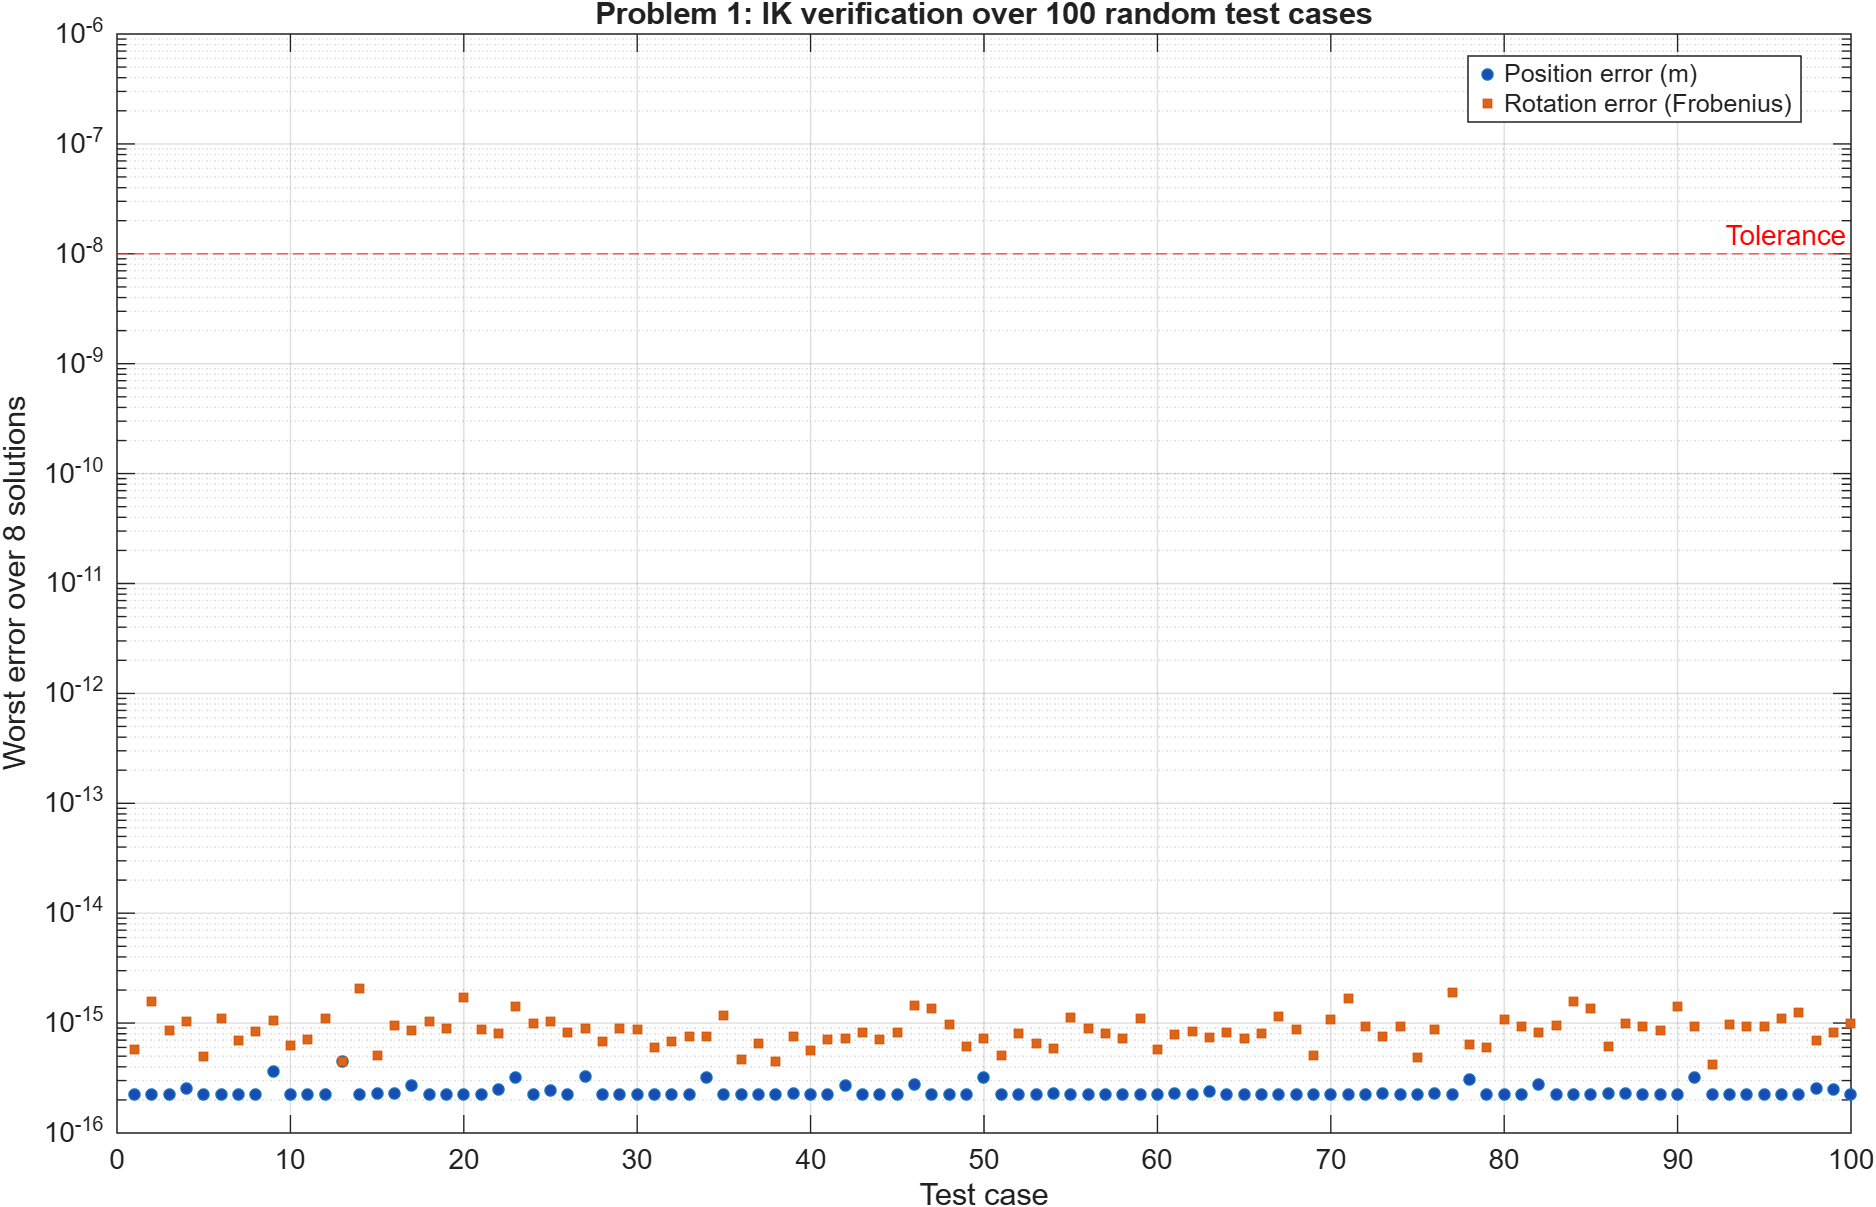
\includegraphics[width=\textwidth]{Figures/Problem1ErrorFigure.png}
\caption{Worst position and rotation error over the 8 IK solutions for each of the 100 random test cases.}
\end{figure}

% ====================================================
% APPENDIX A: CODE
% ====================================================
\newpage
\section*{Appendix A: Code}

% Listings are skipped until the code file exists, so a missing file cannot break the build.
\newcommand{\codelisting}[2]{%
    \IfFileExists{../Code/#1}{\lstinputlisting[language=#2, caption={#1}]{"../Code/#1"}}%
    {\noindent\textcolor{gray!60}{\itshape [#1 not yet written]}}%
}
\newcommand{\funclisting}[2]{%
    \IfFileExists{../../../Functions/#1}{\lstinputlisting[language=#2, caption={#1}]{"../../../Functions/#1"}}%
    {\noindent\textcolor{gray!60}{\itshape [#1 not yet written]}}%
}

\subsection*{Problem 1}\label{app:code:problem1}
\codelisting{Problem1.m}{Matlab}

\newpage
\subsection*{ikABB.m}\label{app:code:ikabb}
\codelisting{ikABB.m}{Matlab}

\newpage
\subsection*{Problem 1 (zero-angle figure)}\label{app:code:problem1fig}
\codelisting{Problem1Figure.m}{Matlab}

\newpage
\subsection*{dhTransform.m}
\noindent\textit{dhTransform.m calls the custom \texttt{rotZ} and \texttt{rotX} functions below (both take radians), not MATLAB's built-in \texttt{rotz}/\texttt{rotx} (which take degrees).}
\funclisting{dhTransform.m}{Matlab}

\newpage
\subsection*{rotZ.m}
\funclisting{rotZ.m}{Matlab}

\newpage
\subsection*{rotX.m}
\funclisting{rotX.m}{Matlab}

\newpage
\subsection*{fkChain.m}
\funclisting{fkChain.m}{Matlab}

% ====================================================
% APPENDIX B: HAND CALCULATIONS
% ====================================================
\newpage
\section*{Appendix B: Hand Calculations}\label{app:hand}

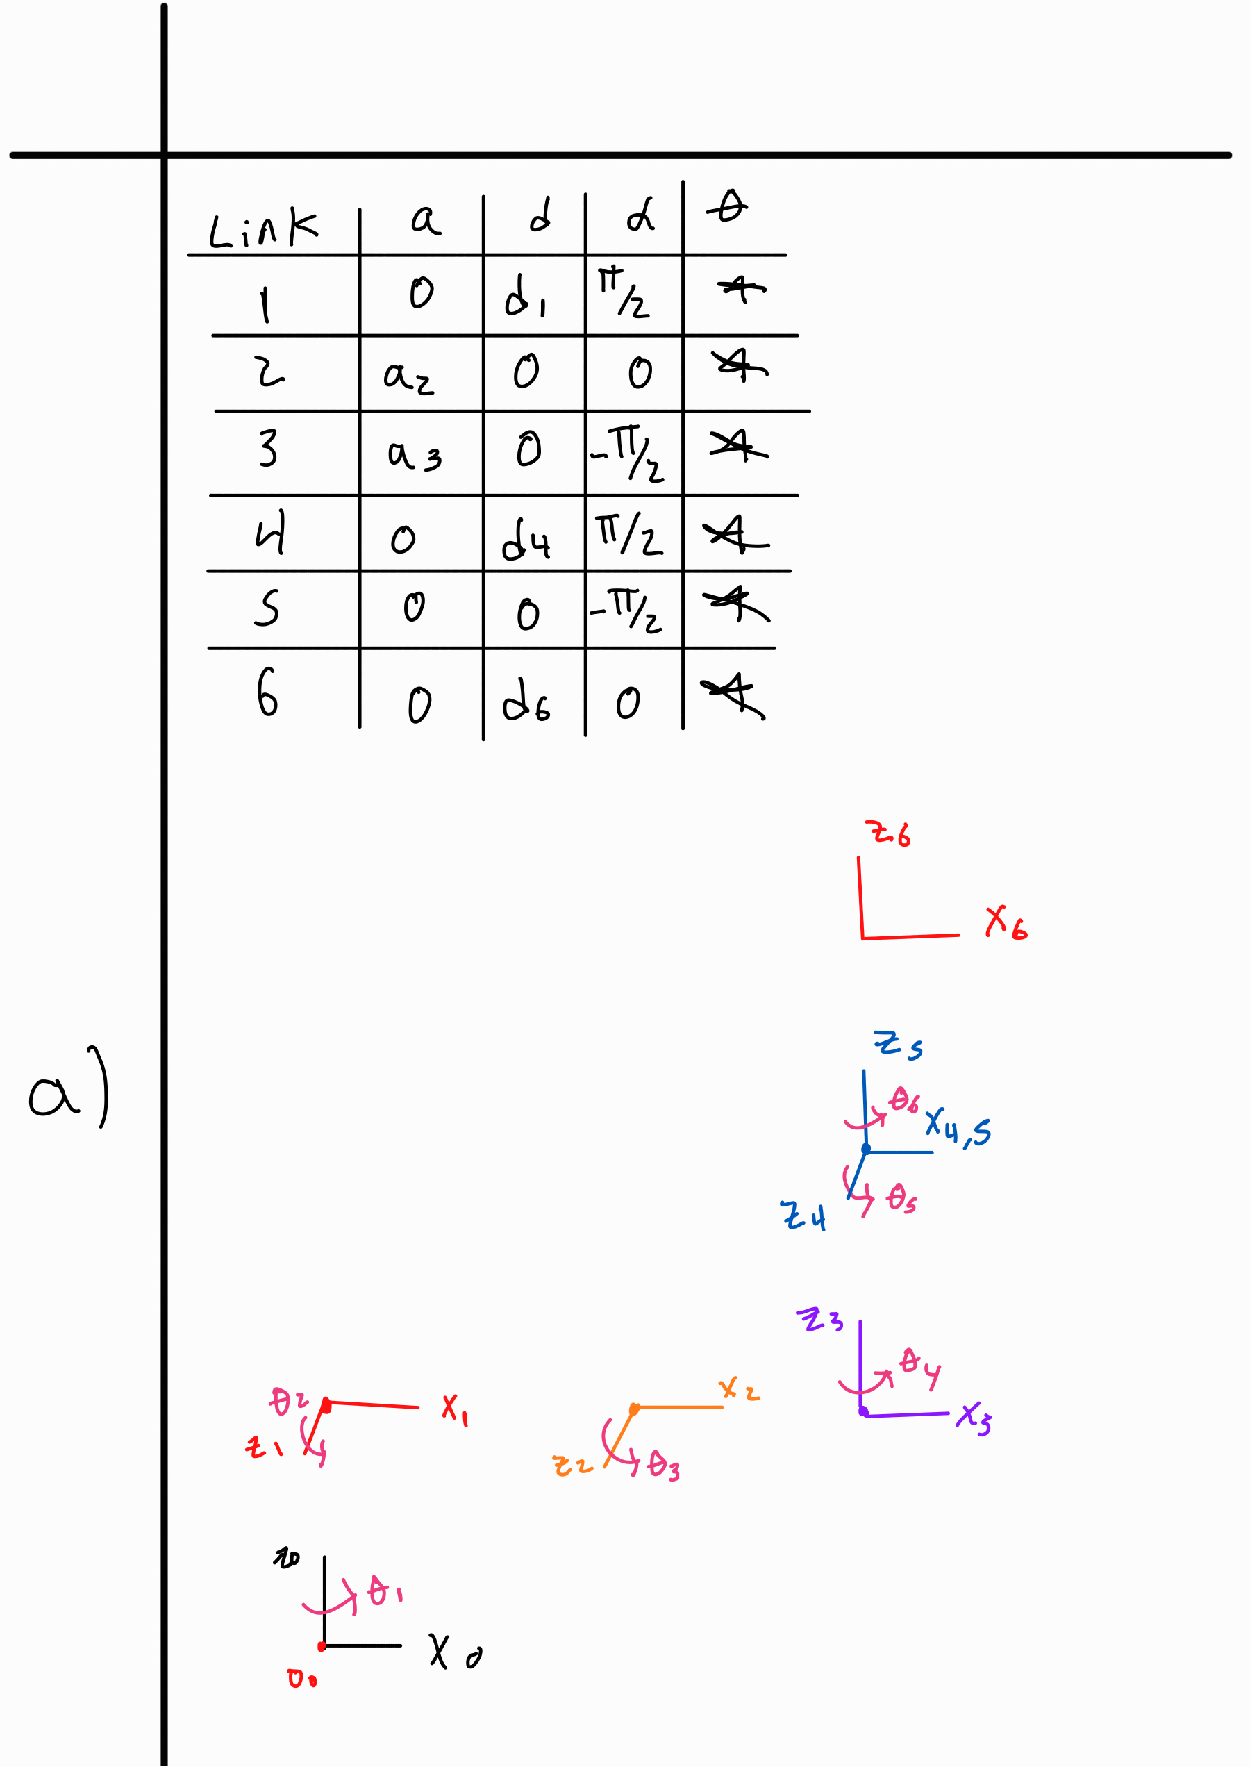
\includepdf[pages=-, pagecommand={\thispagestyle{plain}}, scale=0.9]{../Homework_5_hand_calcs.pdf}

\end{document}
